\documentclass[aps,prd,twocolumn,nofootinbib,superscriptaddress]{revtex4-2}

\usepackage{amsmath,amssymb}
\usepackage{graphicx}
\usepackage{booktabs}
\usepackage{longtable}
\usepackage{hyperref}

\begin{document}

\title{Deformation-Stable Ordering of CP-Phase Admission in Constrained Integer Carriers}

\author{Marvin L. Gentry}
\affiliation{Independent Researcher}

\date{\today}

\begin{abstract}
We define a constrained discrete phase carrier $K_\Lambda\subset\mathbb{Z}_N$ generated by weighted integer combinations modulo $N$ subject to primitivity and a bounded weighted length $\Lambda$. The carrier coverage $|K_\Lambda|/N$ grows monotonically with $\Lambda$ and saturates at a finite cutoff $\Lambda_{\rm sat}$. For a target CP-violating phase $\delta$, we define the admission cutoff $\Lambda_{\rm adm}$ as the smallest $\Lambda$ for which the minimal circular phase distance satisfies $d_{\min}(\Lambda;\delta)\le \Delta$. The dimensionless ratio $\eta=\Lambda_{\rm adm}/\Lambda_{\rm sat}$ enables scale-free comparison across different $N$ and across carrier deformations. Applying this construction uniformly to the CKM phase and to representative PMNS phases (normal and inverted ordering), we find a deformation-stable ordering
$\eta_{\rm CKM}<\eta_{\rm PMNS}^{\rm IO}<\eta_{\rm PMNS}^{\rm NO}$,
with all admissions occurring well below saturation. This hierarchy indicates a structural ordering in admission depth independent of carrier scale.
\end{abstract}

\maketitle

\section{Introduction}

CP violation in the Standard Model is encoded in rephasing-invariant phases of the quark and lepton mixing matrices. While the quark-sector CP phase is precisely measured, the leptonic CP phase remains less constrained and depends on the neutrino mass ordering. Rather than proposing a dynamical origin for these phases, this work addresses a structural question: when identical discrete constraints are imposed, how deeply must a carrier be populated before each physical CP phase is admitted?

\section{Discrete phase carrier}

We consider discrete phases
\begin{equation}
\theta_k=\frac{2\pi k}{N},\qquad k\in\mathbb{Z}_N,
\end{equation}
and generate admissible residues via
\begin{equation}
k\equiv w_1 a+w_2 b+w_3 c\pmod N,
\end{equation}
subject to
\begin{align}
w_1|a|+w_2|b|+w_3|c| &\le \Lambda,\\
\gcd(a,b,c)&=1,\\
(a,b,c)&\neq (0,0,0).
\end{align}
For fixed $(N,\mathbf{w})$ and cutoff $\Lambda$, the admissible residue set $K_\Lambda\subset\mathbb{Z}_N$ defines the carrier coverage
\begin{equation}
C(\Lambda)=\frac{|K_\Lambda|}{N}.
\end{equation}
As $\Lambda$ increases, $C(\Lambda)$ grows monotonically until saturation.

\section{Admission metric and normalized depth}

Agreement with a target phase $\delta$ is measured using the circular distance on $S^1$,
\begin{equation}
d(\theta,\delta)=\min_{n\in\mathbb{Z}}|\theta-\delta+2\pi n|.
\end{equation}
For a given carrier $K_\Lambda$, define
\begin{equation}
d_{\min}(\Lambda;\delta)=\min_{k\in K_\Lambda} d(\theta_k,\delta).
\end{equation}
The \emph{admission cutoff} $\Lambda_{\rm adm}$ is the smallest $\Lambda$ such that
\begin{equation}
d_{\min}(\Lambda;\delta)\le \Delta,
\end{equation}
for a fixed tolerance $\Delta$.

To enable comparison across different $N$ and scaffold choices, we define the dimensionless \emph{normalized admission depth}
\begin{equation}
\eta=\frac{\Lambda_{\rm adm}}{\Lambda_{\rm sat}},
\end{equation}
where $\Lambda_{\rm sat}$ is the smallest cutoff for which $C(\Lambda)=1$.

\subsection{Computation}

For fixed $(N,\mathbf{w})$, we enumerate all integer triples $(a,b,c)\in\mathbb{Z}^3$ satisfying $\gcd(a,b,c)=1$ and
$w_1|a|+w_2|b|+w_3|c|\le \Lambda$, collecting residues
$k\equiv w_1 a+w_2 b+w_3 c\pmod N$ to form $K_\Lambda$.
The saturation cutoff $\Lambda_{\rm sat}$ is the smallest $\Lambda$ for which $|K_\Lambda|=N$.
For a target phase $\delta$, the admission cutoff $\Lambda_{\rm adm}$ is the smallest $\Lambda$ satisfying the distance criterion above.
All results are deterministic given $(N,\mathbf{w},\delta,\Delta)$.

\section{Inputs and deformation set}

We use the central values
\begin{align}
\delta_{\rm CKM} &= 65.718^\circ,\\
\delta_{\rm PMNS}^{\rm NO} &= 177^\circ,\\
\delta_{\rm PMNS}^{\rm IO} &= 285^\circ,
\end{align}
with tolerances $\Delta_{\rm CKM}=1.5^\circ$ and $\Delta_{\rm PMNS}=10^\circ$.

To test deformation stability we evaluate the integer scaffolds
\begin{equation}
(8,15,24),\quad (7,15,24),\quad (8,14,25),\quad (9,15,23),
\end{equation}
for representative values $N\in\{60,100,120,180\}$.

\section{Results}

\paragraph{Result.}
Across all tested $(N,\mathbf{w})$, we observe a strict ordering in normalized admission depth,
\begin{equation}
\eta_{\rm CKM}<\eta_{\rm PMNS}^{\rm IO}<\eta_{\rm PMNS}^{\rm NO}.
\end{equation}
Because $\eta$ is defined relative to the saturation scale $\Lambda_{\rm sat}$, this ordering is insensitive to absolute carrier scale and persists under scaffold deformations that modify coverage growth.

\begin{table}[t]
\centering
\caption{Representative normalized admission depths for $N=120$. The complete table across all tested $(N,\mathbf{w})$ is provided in Appendix~\ref{app:fulltable}.}
\label{tab:rep}
\begin{ruledtabular}
\begin{tabular}{cccc}
Weights & $\eta_{\rm CKM}$ & $\eta_{\rm PMNS}^{\rm IO}$ & $\eta_{\rm PMNS}^{\rm NO}$ \\
\hline
8-15-24 & 0.328 & 0.198 & 0.483 \\
7-15-24 & 0.244 & 0.244 & 0.633 \\
8-14-25 & 0.220 & 0.220 & 0.570 \\
9-15-23 & 0.667 & 0.225 & 0.549 \\
\end{tabular}
\end{ruledtabular}
\end{table}

\begin{figure}[t]
\centering
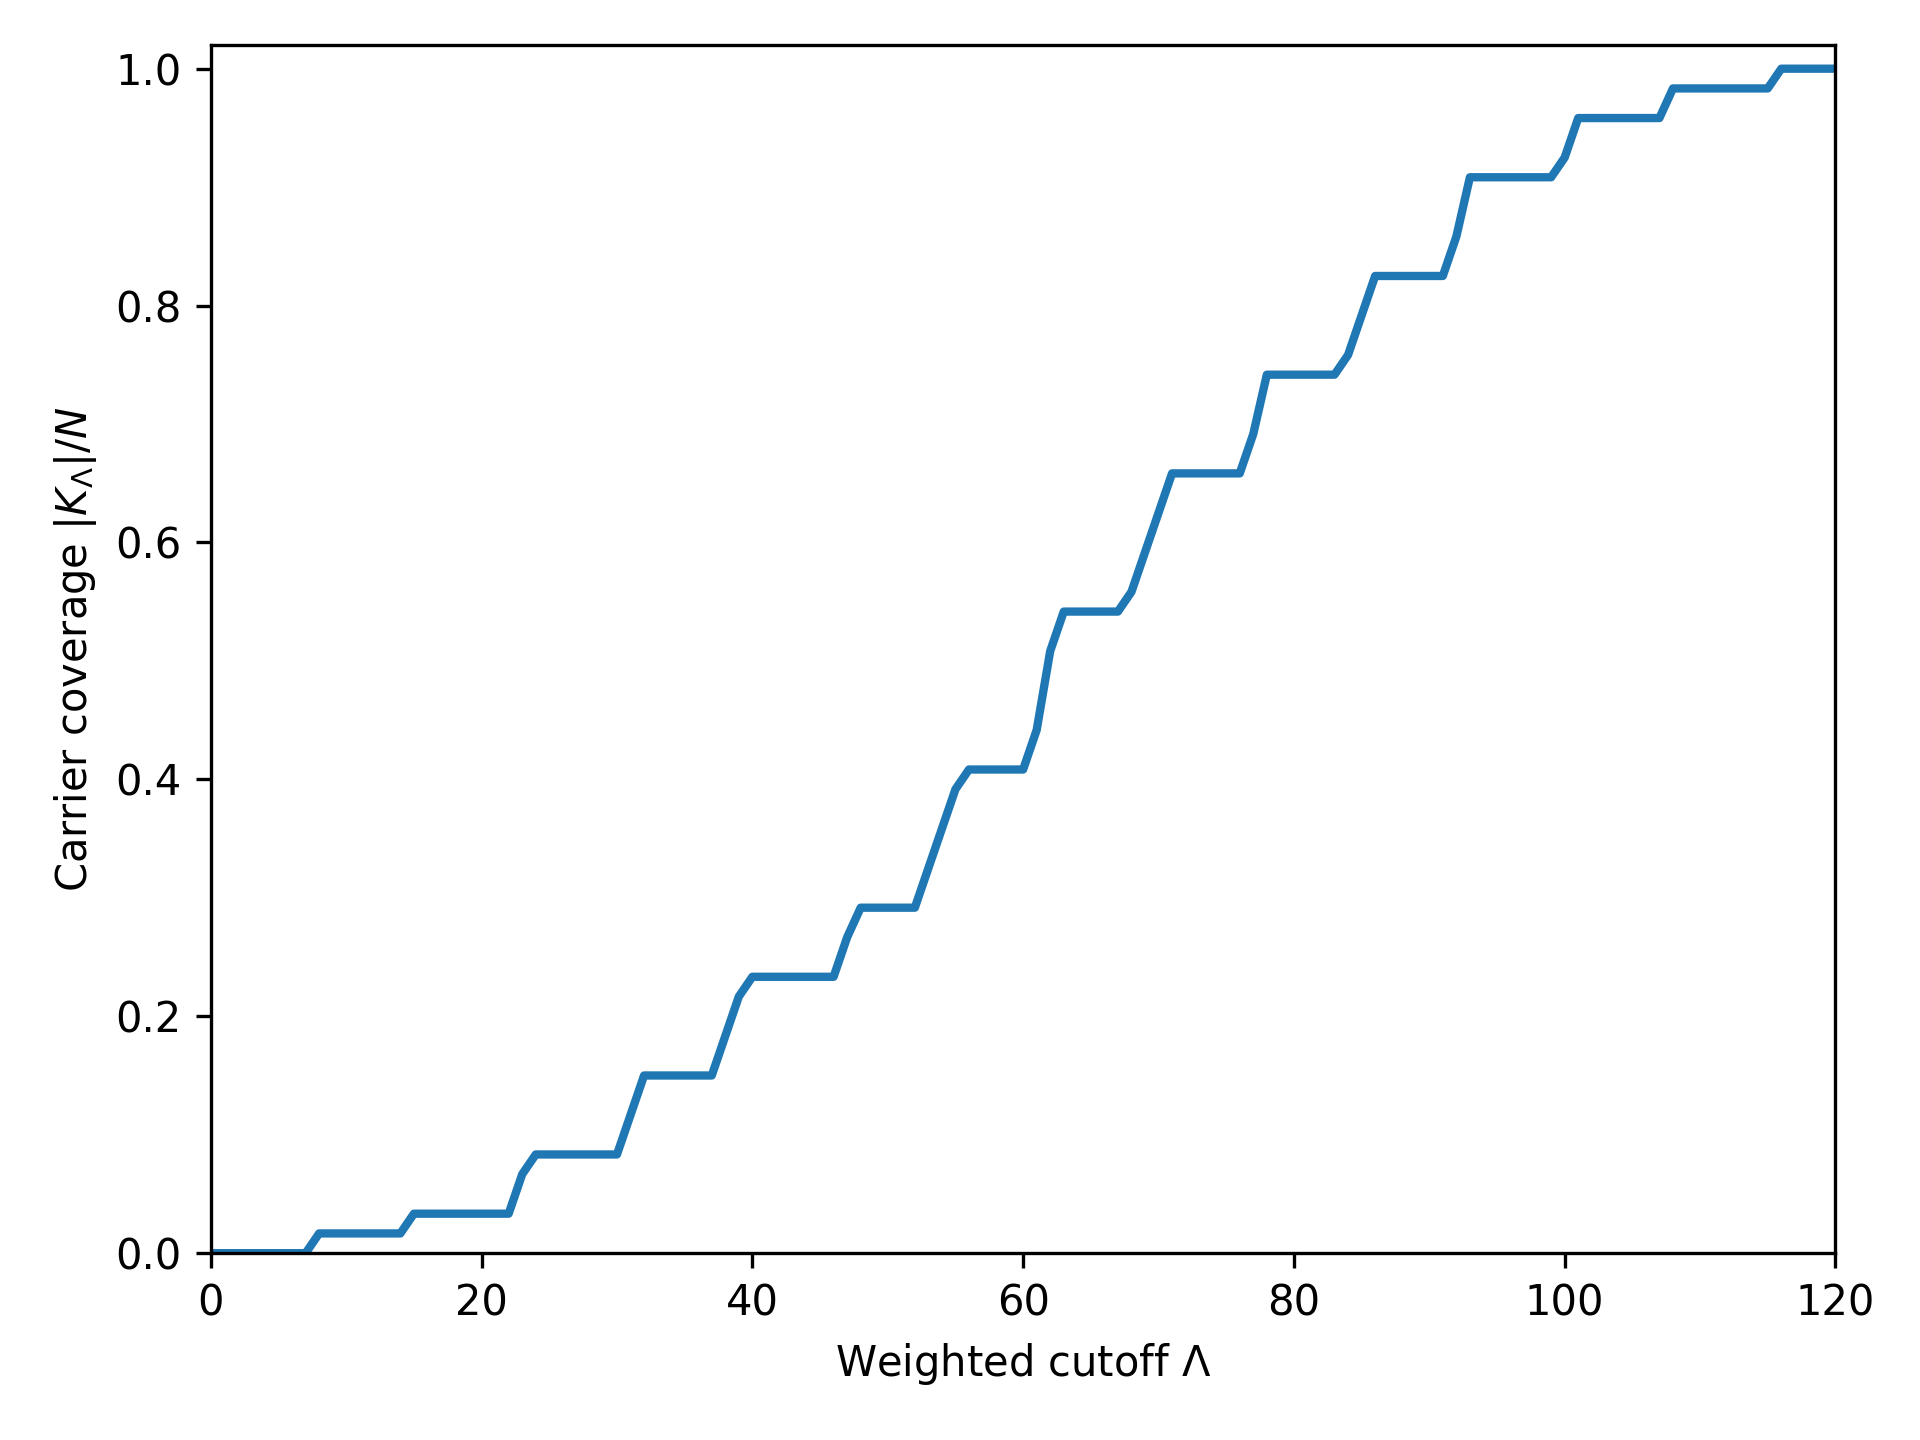
\includegraphics[width=\linewidth]{fig1_carrier_coverage_N120.png}
\caption{Carrier coverage $|K_\Lambda|/N$ versus weighted cutoff $\Lambda$ for $N=120$ (baseline scaffold $\mathbf{w}=(8,15,24)$). Admission of the CKM and PMNS target phases occurs well below saturation, indicating that the observed ordering is not a saturation artifact.}
\label{fig:coverage}
\end{figure}

\begin{figure}[t]
\centering
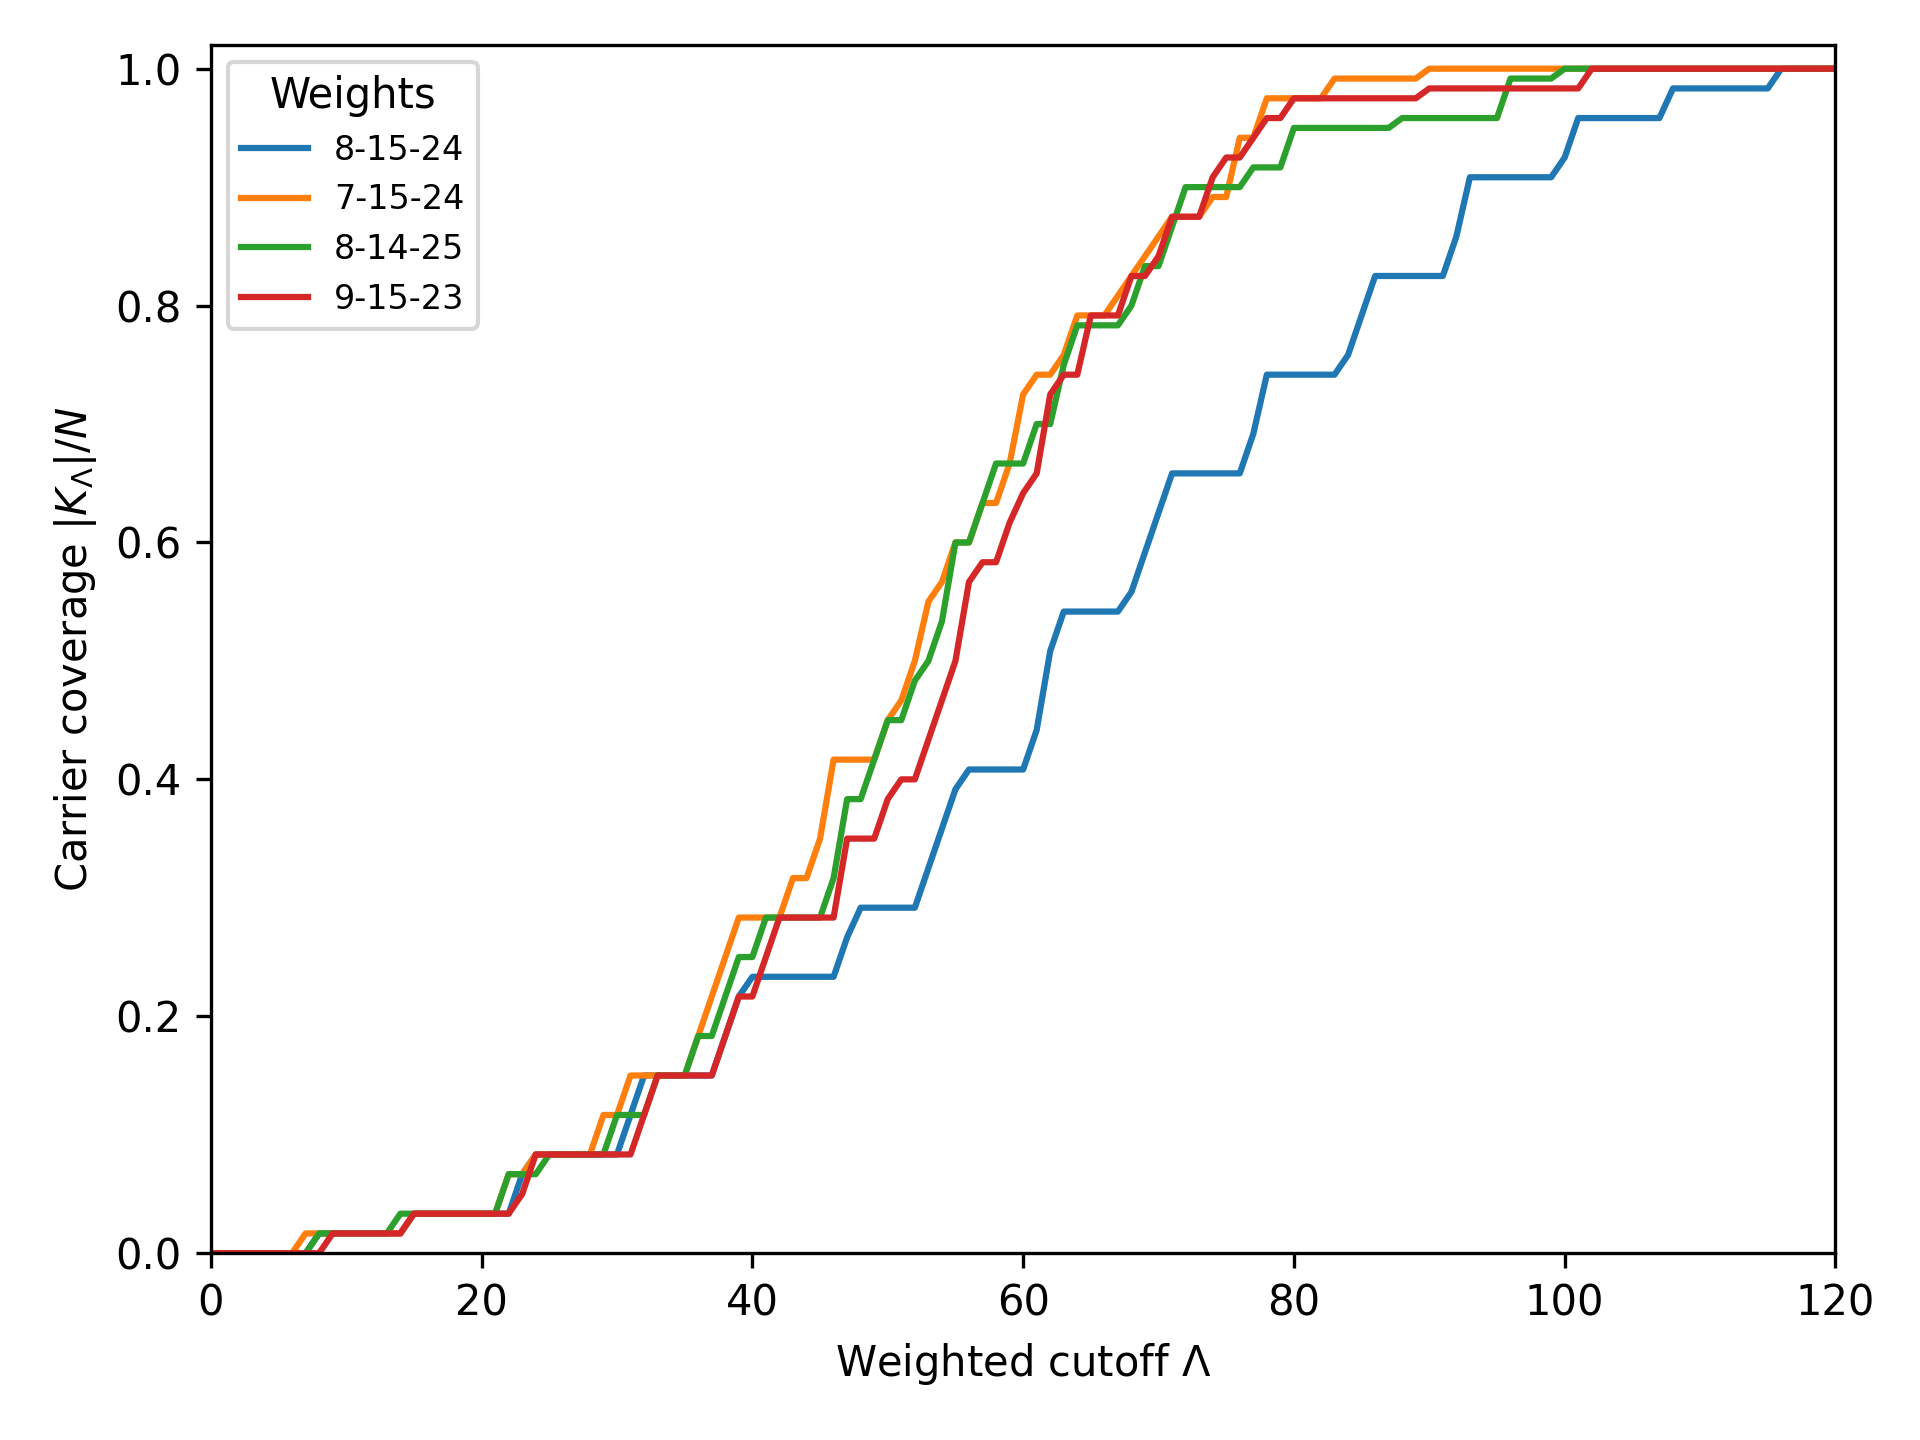
\includegraphics[width=\linewidth]{fig2_deformation_stability_N120.png}
\caption{Coverage curves for $N=120$ under small scaffold deformations. Similar growth and comparable saturation scales support robustness of $\eta$ as a comparative invariant.}
\label{fig:deformation}
\end{figure}

\section{Conclusion and falsifiability}

We identify a deformation-stable, scale-invariant ordering governing the admission of CP-violating phases into constrained discrete carriers. Under identical structural constraints, the CKM phase is admitted at lower normalized depth than representative leptonic phases, with the PMNS normal-ordering target requiring the deepest carrier penetration.

This framework is falsifiable. Observation of a leptonic CP phase that admits at lower normalized depth than the CKM phase under the same carrier constraints would invalidate the ordering identified here.

\appendix
\section{Full deformation table}
\label{app:fulltable}

\begin{longtable}{cccccc}
\caption{Admission cutoff $\Lambda_{\mathrm{adm}}$, saturation cutoff $\Lambda_{\mathrm{sat}}$, and normalized depth $\eta$ across all tested $(N,\mathbf{w})$.}\\
\toprule
Weights & $N$ & Sector & $\Lambda_{\mathrm{adm}}$ & $\Lambda_{\mathrm{sat}}$ & $\eta$ \\
\midrule
\endfirsthead

\toprule
Weights & $N$ & Sector & $\Lambda_{\mathrm{adm}}$ & $\Lambda_{\mathrm{sat}}$ & $\eta$ \\
\midrule
\endhead

\midrule
\multicolumn{6}{r}{\emph{Continued on next page}}\\
\endfoot

\bottomrule
\endlastfoot

8-15-24 & 60 & CKM & 71 & 86 & 0.826 \\
8-15-24 & 60 & PMNS\_NO & 31 & 86 & 0.360 \\
8-15-24 & 60 & PMNS\_IO & 47 & 86 & 0.547 \\
8-15-24 & 100 & CKM & 78 & 110 & 0.709 \\
8-15-24 & 100 & PMNS\_NO & 47 & 110 & 0.427 \\
8-15-24 & 100 & PMNS\_IO & 23 & 110 & 0.209 \\
8-15-24 & 120 & CKM & 38 & 116 & 0.328 \\
8-15-24 & 120 & PMNS\_NO & 56 & 116 & 0.483 \\
8-15-24 & 120 & PMNS\_IO & 23 & 116 & 0.198 \\
8-15-24 & 180 & CKM & 63 & 138 & 0.457 \\
8-15-24 & 180 & PMNS\_NO & 84 & 138 & 0.609 \\
8-15-24 & 180 & PMNS\_IO & 38 & 138 & 0.275 \\
7-15-24 & 60 & CKM & 59 & 64 & 0.922 \\
7-15-24 & 60 & PMNS\_NO & 29 & 64 & 0.453 \\
7-15-24 & 60 & PMNS\_IO & 43 & 64 & 0.672 \\
7-15-24 & 100 & CKM & 60 & 90 & 0.667 \\
7-15-24 & 100 & PMNS\_NO & 50 & 90 & 0.556 \\
7-15-24 & 100 & PMNS\_IO & 22 & 90 & 0.244 \\
7-15-24 & 120 & CKM & 22 & 90 & 0.244 \\
7-15-24 & 120 & PMNS\_NO & 57 & 90 & 0.633 \\
7-15-24 & 120 & PMNS\_IO & 22 & 90 & 0.244 \\
7-15-24 & 180 & CKM & 63 & 102 & 0.618 \\
7-15-24 & 180 & PMNS\_NO & 84 & 102 & 0.824 \\
7-15-24 & 180 & PMNS\_IO & 36 & 102 & 0.353 \\
8-14-25 & 60 & CKM & 39 & 88 & 0.443 \\
8-14-25 & 60 & PMNS\_NO & 30 & 88 & 0.341 \\
8-14-25 & 60 & PMNS\_IO & 14 & 88 & 0.159 \\
8-14-25 & 100 & CKM & 46 & 100 & 0.460 \\
8-14-25 & 100 & PMNS\_NO & 47 & 100 & 0.470 \\
8-14-25 & 100 & PMNS\_IO & 22 & 100 & 0.220 \\
8-14-25 & 120 & CKM & 22 & 100 & 0.220 \\
8-14-25 & 120 & PMNS\_NO & 57 & 100 & 0.570 \\
8-14-25 & 120 & PMNS\_IO & 22 & 100 & 0.220 \\
8-14-25 & 180 & CKM & 33 & 104 & 0.317 \\
8-14-25 & 180 & PMNS\_NO & 84 & 104 & 0.808 \\
8-14-25 & 180 & PMNS\_IO & 33 & 104 & 0.317 \\
9-15-23 & 60 & CKM & 65 & 65 & 1.000 \\
9-15-23 & 60 & PMNS\_NO & 32 & 65 & 0.492 \\
9-15-23 & 60 & PMNS\_IO & 32 & 65 & 0.492 \\
9-15-23 & 100 & CKM & 100 & 100 & 1.000 \\
9-15-23 & 100 & PMNS\_NO & 47 & 100 & 0.470 \\
9-15-23 & 100 & PMNS\_IO & 23 & 100 & 0.230 \\
9-15-23 & 120 & CKM & 68 & 102 & 0.667 \\
9-15-23 & 120 & PMNS\_NO & 56 & 102 & 0.549 \\
9-15-23 & 120 & PMNS\_IO & 23 & 102 & 0.225 \\
9-15-23 & 180 & CKM & 33 & 110 & 0.300 \\
9-15-23 & 180 & PMNS\_NO & 84 & 110 & 0.764 \\
9-15-23 & 180 & PMNS\_IO & 33 & 110 & 0.300 \\


\end{longtable}

\end{document}
